\section{Módulo de análisis}

El módulo de análisis, como ya se ha comentado, es el encargado de, dada una imagen dada y una configuración de entrada, producir un archivo XML con la lista de polígonos que componen la imagen. Esta lista debe componer una nueva imagen lo más fiel posible a la imagen de entrada, teniendo en cuenta los ajustes especificados en el archivo de configuración.\\

Este módulo hace un gran uso de la librería externa OpenCV, de la cual se ayuda tanto para tratar imágenes como para componer formas y polígonos.

\subsection{Vista de implementación}

La estructura general del módulo se ve en la Figura~\ref{fig:diagramaclasesPHIC}.\\

		\begin{figure}[htbp]
		\centering
		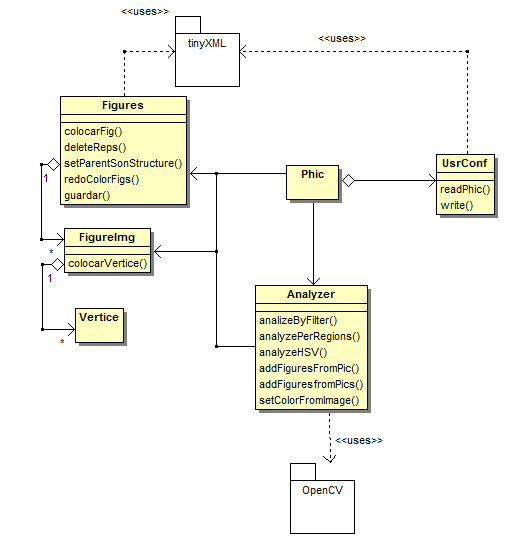
\includegraphics[scale=0.6]{graphics/diagramaclasesPHIC.png}
		\caption{Vista de las clases del módulo de anális}
		\label{fig:diagramaclasesPHIC}
		\end{figure}
		
En ella, se pueden observar las siguientes clases:\\

\begin{itemize}

	\item \textbf{Phic:} Se trata de la clase que controla la completa ejecución de este módulo. Se ocupa de coordinar el resto de clases para que realicen las operaciones requeridas para completar el análisis.
	
	\item \textbf{Analizer:} realiza todas las operaciones de análisis y se comunica con la librería OpenCV.
	
	\item \textbf{UsrConf:} como se explica en posteriores secciones, es una clase común que se ocupa de la lectura de los archivos de configuración.
	
	\item \textbf{Figures:} el módulo de análisis utiliza de forma directa la clase Figures anteriormente mencionada. Se muestran en el diagrama los métodos que llevan a cabo las funcionalidades necesarias para la ejecución de este módulo.
	
	\item \textbf{FigureImg:} se trata de una especificación de la clase Figure, que toma como padre.
	
	\item \textbf{Vertice:} como se comenta en previas secciones, representa cada uno de los vértices que componen un polígono. 
	
	\item \textbf{TinyXML:} Se trata de un paquete externo de código libre que permite generar y manipular archivos XML.
	
	
\end{itemize}
			
El flujo de ejecución de un análisis cualquiera realizado con este módulo se ve en la Figura~\ref{fig:diagramaflujoPHIC}. En él, se observa cómo es Analyzer la que se comunica con OpenCV para realizar las opciones necesarias, ordenadas por Phic.\\

		\begin{figure}[htbp]
		\centering
		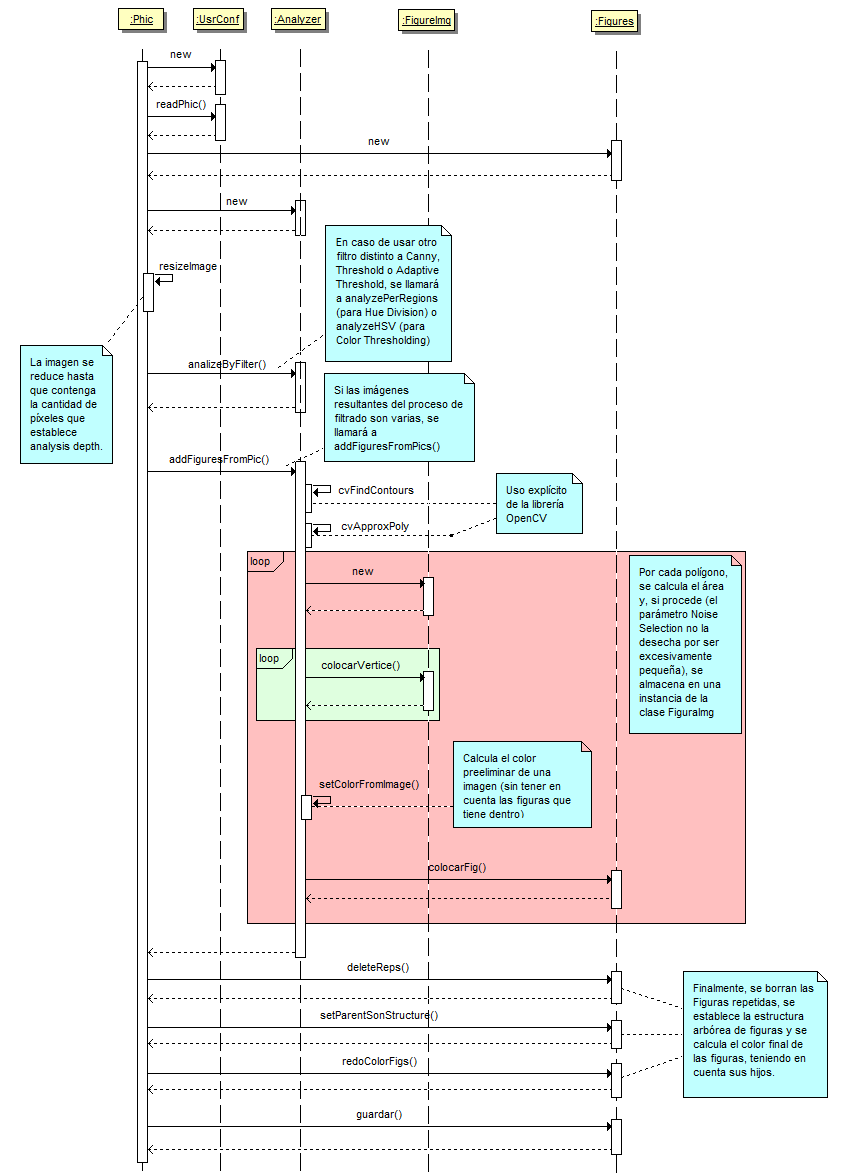
\includegraphics[scale=0.47]{graphics/diagramaflujoPHIC.png}
		\caption{Flujo de ejecución del módulo de anális}
		\label{fig:diagramaflujoPHIC}
		\end{figure}
		
\subsection{Vista de despliegue}
\todo{puede que sobre porque es obvio y UBERrepetitivo, pero es para que se vea que opencv está como dll ahí}
		
Por último, la vista final del módulo como paquetes se ve en la Figura~\ref{fig:diagramapaquetesPHIC}.\\

		\begin{figure}[htbp]
		\centering
		
\includegraphics[scale=0.47]{graphics/todo.png}
		\caption{Diagrama de paquetes del módulo de anális}
		\label{fig:diagramapaquetesPHIC}
		\end{figure}
		
El sistema se basa en la librería externa OpenCV para relizar sus funciones.